\subsubsection{The FRODO platform}

Although the TTA approach to fault-tolerant execution of control applications has been developed and matured over many years, its current manifestation only as a hardware specific platform restricts the flexibility and portability of possible applications developed using the toolchain.  These obstacles motivated a second deployment platform for the toolchain that offered the same deterministic execution of the TT MoC with off-the-shelf components and a hardware/software independent platform API.  The resulting platform uses an abstract virtual machine, called FRODO, for executing TT control tasks of high-confidence systems coupled with a message controller that provides the TT transmission of data message across networked nodes, all of which is implemented using readily available infrastructure.

\subsubsection*{Architecture}

This platform's implementation architecture is based on logical separation principles similar to those of other TT platforms like Giotto \cite{henzinger01giotto} and TTA \cite{kopetz:2001-22}:  the periodic execution of control tasks is determined solely by the passage of time and the current operational mode of the system, i.e. events such as the arrival of new data messages do not affect the timely task execution.  Accordingly, only the most recent data values, representative of some control signals, are relevant to calculations performed by TT tasks; therefore, a globally shared memory construct is used to read and update data throughout execution.  The resulting architecture is provided below in Figure~\ref{fig:FRODOArch}.  In the figure, bidirectional arrows represent the flow of data throughout the system whereas the unidirectional arrows indicate the sending of relevant events.  The current platform implementation uses embedded PC-s running on Linux 2.6.x kernels and standard Ethernet UDP network for communication.

\begin{figure}[h]
  \centering
   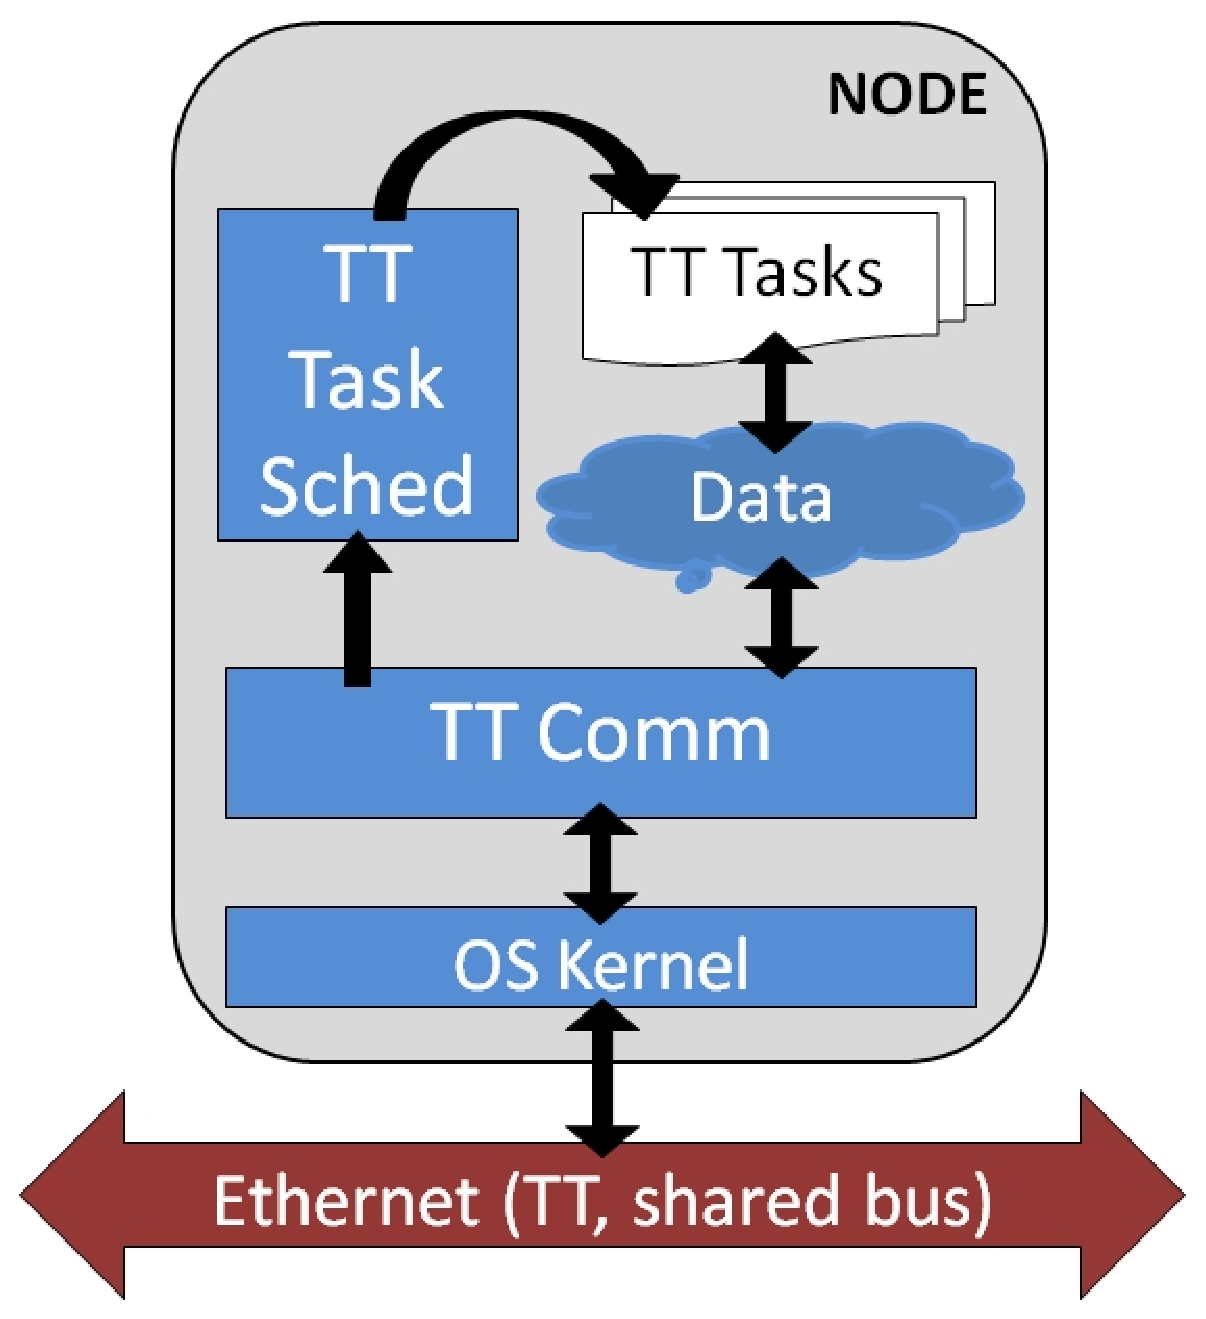
\includegraphics[width=0.5\columnwidth]{FRODOArch}
   \caption{FRODO implementation architecture.}
   \label{fig:FRODOArch}
\end{figure}

\subsubsection*{Time-triggered communication}
Maintaining low overhead and platform independence for the message controller was necessary to making this platform as portable as possible.  Accordingly, the communication controller expects only a shared bus network configuration for connecting all of the nodes in the system and a library of methods that provide the basic functionality for sending and receiving messages.  Unlike the TTP platform described above but similar to the TTP/A protocol \cite{kopetz:2000-23}, this platform is not yet robust enough to provide a fault-tolerant synchronization approach for maintaining a global clock; instead, a designated communications controller in the system is responsible for initially verifying all of the expected nodes are connected to the network before starting execution and synchronizing the start of the each message schedule round with all of the nodes.  All other nodes on the network will not begin executing unless confirmation is received that all nodes are present at startup, and they will also fail to start a new schedule round unless the proper synchronization message is received.

Based on the previous discussion of the properties of the TT MoC, the certification/verification of distributed control systems is contingent upon the deployed system's ability to accurately follow a fixed message schedule; therefore, the use of a TT capable message controller is paramount to this platform's applicability for systems developed using the toolchain.  Like the TTP approach, a static message schedule is generated offline, passed as an input to the platform, and cyclically iterated throughout the execution; however, the format of the message schedule is not identical to that used in TTP.  TTP requires the use of a strict TDMA format where all nodes have a scheduled time-slot for transmitting messages in each round.  Conversely, this platform does not place any minimum or maximum on the amount of data that can be sent from a node in a round except those constraints that maintain the feasibility of the message schedule.  Instead, the static message schedule specifies exactly which node sends a message at an exact scheduled offset with respect to the start of the schedule round.  Each schedule round is one hyperperiod long, and the hyperperiod is of fixed duration.  A node will be allotted no messages/slots if it is not expected to transmit any data within a schedule round.  If a message is expected to be sent with a frequency greater than one within a round, it will be listed as many times in the schedule as it is expected with each appropriate scheduled transmission time.  The length of each message, in bytes, is also indicated in the message schedule.

The current steps for establishing and maintaining TT communication across a network of nodes implemented using this platform proceeds in the following steps:
\begin{enumerate}
\setlength{\itemsep}{1pt}
\setlength{\parskip}{0pt}
\setlength{\parsep}{0pt}
\item Discovery of all nodes required by the implementation
\item Transmission of hyperperiod start signal (beginning of schedule execution)
\item Transmission of data messages in their strict scheduled order
\item End of hyperperiod is reached
\item Repeat starting from step 2 or terminate execution
\end{enumerate}
Obviously, while each individual node is preparing to transmit its scheduled data messages, it must also be configured to receive broadcast messages from other controllers in order to maintain the most up-to-date data set.  Each outgoing message includes a message indicator such that the receivers can quickly locate the appropriate memory location to update with the received value.  A snapshot of the activity on the communication network over two hyperperiods of the message schedule is provided in Figure~\ref{fig:FRODOTimeline}.

\begin{figure}[h]
   \centering
   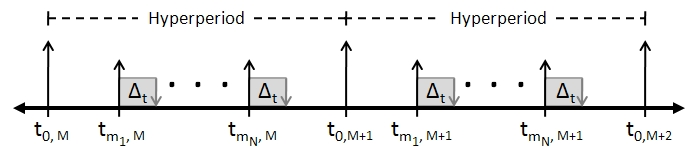
\includegraphics[width=0.95\columnwidth]{FRODOTimeline}
   \caption{Activity timeline across time-triggered network.}
   \label{fig:FRODOTimeline}
\end{figure}

\subsubsection*{Time-triggered task execution}
The application code that provides the functionality of the individual toolchain components is generated completely agnostic to the choice of target platform(s).  Instead, the tasks that contain the application code of the components provide only timing information regarding their execution and require access to the data relevant to the control calculations they perform.  Accordingly, the platform's task scheduler need only expose an interface fitting the tasks' needs and have the capability to invoke and terminate task execution in order to provide precise controller execution.  FRODO is such an abstract, platform-independent executive (virtual machine) responsible for providing the necessary TT execution of control tasks on this platform.

Most commonly, digital implementations of controllers operate in a periodic fashion---sampling control signals, computing the next control signal and the current state of the system, and performing an actuation based on the computations.  Likewise, the task scheduler of FRODO is responsible for initiating the periodic execution of the control tasks based on a static task execution schedule initially passed as input to the system.  The current implementation of FRODO does not allow the preemption of tasks, i.e. only one periodic control task is released for execution at any given time.  In order to maintain the timely execution of the control tasks according to the schedule, FRODO is also responsible for terminating executing tasks that have yet to finish prior to reaching their worst-case execution time (WCET).
The task schedule for a node is similar to the message schedule mentioned in the preceding section: each task invocation is explicitly listed in the schedule with its appropriate release time with respect to the start of the schedule and the task schedule has the same length or hyperperiod as the message schedule.  Synchronizing the execution of the task schedule with the message schedule maintains the controller correctness with respect to the current control signals; therefore, each new round of the task schedule has to be initiated by the arrival of an event from the underlying communication controller indicating that a new schedule round is beginning.  If no such event is received, the control tasks will not be released for execution.

Only as a scheduled task begins and (properly) ends execution, it will require the necessary access to the globally shared memory to read/update the control signal data used throughout the system.  Accordingly, FRODO provides two methods for performing such operations; however, internally FRODO must use proper access-control locks to ensure that it is not updating values concurrently with the message controller.
